\documentclass{article}

% Recommended, but optional, packages for figures and better typesetting:
\usepackage{microtype}
\usepackage{graphicx}
\usepackage{subfigure}
\usepackage{booktabs} % for professional tables
\usepackage{multirow}
% hyperref makes hyperlinks in the resulting PDF.
% If your build breaks (sometimes temporarily if a hyperlink spans a page)
% please comment out the following usepackage line and replace
% \usepackage{icml2021} with \usepackage[nohyperref]{icml2021} above.
\usepackage{hyperref}
\usepackage{enumitem}
\usepackage{todonotes}
\usepackage[flushleft]{threeparttable}
% Attempt to make hyperref and algorithmic work together better:
\newcommand{\theHalgorithm}{\arabic{algorithm}}


\usepackage[accepted]{icml2021}

\icmltitlerunning{Deliverer Employment Effects on Profit for Delivery Companies Using Multi Agent Modeling}
\begin{document}


    \twocolumn[
        \icmltitle{Deliverer Employment Effects on Profit for Delivery Companies Using Multi Agent Modeling}

        \begin{icmlauthorlist}
            \icmlauthor{Evert van Kammen (Student nr. 850227069)}{ou}
        \end{icmlauthorlist}

        \icmlaffiliation{ou}{Open Universiteit}

        \icmlcorrespondingauthor{E van Kammen}{evert@evkammen.nl}

% You may provide any keywords that you
% find helpful for describing your paper; these are used to populate
% the "keywords" metadata in the PDF but will not be shown in the document
        \icmlkeywords{}

        \vskip 0.3in
    ]

    \printAffiliationsAndNotice

% the background and issues of your proposed research,
% identify your discipline,
% a short literature review,
% a summary of key debates and developments in the field.


\section{Introduction}

Food delivery companies, like Uber Eats and Thuisbezorgd.nl, offer a service where customers can order food from restaurants and get the meal delivered at home.
These companies get a fee per delivery and pay deliverers an hourly wage and/or pay them per delivery.

E.g., Uber Eats~\footnote{\url{https://merchants.ubereats.com/gb/en/pricing/}} charges 30\% of the total value of an ordered meal to be paid by the restaurant.
Deliverers get paid per delivery (this is not true in all countries) this consists of a base pay and an optional tip from the customer.
Drivers may decide to take an order or not, they are seen as independent contractors.

Lately delivery companies have had some bad publicity of being unfair and exploiting the deliverers.
In the Netherlands the government calls the status of these deliverers: bogus self-employment.
That is why in the Netherlands delivery companies are forced to hire them as employees with all benefits and pay an hourly wage.
But in other countries they still see them as independent workers and pay them per delivery.

Delivery companies seem to prefer the per-delivery system as they do not have to pay for the time no deliveries are made.
This system may have advantages for the deliverers too, some may make more money if they can make many deliveries.
But, if deliverers don't make enough money they may quit and thus fewer deliveries can be made leading to lesser profits for the delivery companies.

In this research project different scenarios are simulated where deliverers deliver ordered meals to customers.
The scenarios differ in how deliverers are treated: as independent contractors who get paid per delivery and thus may decide to take an order or not versus
deliverers hired as employees where orders are distributed among available deliverers.
In the context of these scenarios the profit of the company will be calculated, also the number of participating restaurants, deliverers and customers will analyse.

This is an economic problem that has both micro and macroeconomic facets.
Microeconomic as it deals with agents that make decisions, e.g., hire deliverers, maximise the delivery companies profit, order food, become a deliverer or deside to stop being a deliverer.
Macroeconomics, because there is a labour market, i.e., the deliverers.

A model will, like in a laboratory setting, include only properties we are interested in and exclude elements like e.g., weather and physical conditions of deliverers.
The tool for building the model is: NetLogo ~\cite{NetLogo2024}.
This is a multi-agent programmable modeling environment.
This environment has been used to create models for many sciences concerning multi-agents (from how viruses spread to how agents act in game theory~\cite{r2019agent}).

Other research projects reported about the food delivery sector using the NetLogo tool.
An existing model for the food delivery context is created by~\cite{ismail2024software}.
This model was used to research the efficiency of food delivery.
The model consists riders, vendors and customers.
The world consists of a 2-dimensional grid where riders have to pick up food from vendors and deliver it to customers.
This project also mentioned some real world rules the 3 types of agents possess.

In another study ~\cite{antelmi2024reliable} NetLogo is compared to other ABM systems and integrations with other programming languages are analysed.

\subsection{Research goals}
The main research goal is to create an Agent Based Model to compare two deliverer employment scenarios in the food delivery industry.

The two main scenarios of interest are:
\begin{itemize}
    \item one, where the deliverers are hired as employees
    \item versus a scenario where deliverers are independent contractors and get paid per delivery
\end{itemize}

During the model building and design, new-found insights will be used in deciding which variables and, if needed, which economic theories to use, and adjust the model as needed.

This first part of the model will be used to find a baseline and will be used to test the model.
This model is the simpler one, at start the certain variables to be used are the number of deliverers and the strategy for delivery distribution.

The second part is based on the first, the main-difference is that the delivers are not hired but paid per delivery, if they make enough money they stay otherwise they stop.
Interesting variables are: the amount paid per delivery, the wage they could earn in a steady job (like in te first part) and the distribution strategy of deliveries.

Thus, the research goals are:
\begin{itemize}
 \item \textbf{Building the above-mentioned model in NetLogo, creating it as a highly abstracted but still believable world.}
 \item \textbf{Finding how the profit for a delivery company varies when using independent contractors versus hiring deliverers as employees.}
\end{itemize}

Answer will be of the kind:

time series: profits over time, averages of multiple runs


\todo[inline]{Write more about this \& author.}




% the theoretical resources to be drawn on,
% the research approach (theoretical framework),
% the research methods appropriate for the proposed research, a discussion of advantages as well as limits of particular approaches and methods.
%! Author = evert
%! Date = 21-7-2024

\section{Research goals}
The main research goal behind this proposal is, finding answers to:

\textbf{How does the profit for delivery companies vary when using independent contractors versus hiring deliverers as employees with an hourly wage? }

An instrument will be built in the form of an Agent Based Model.
Calling it an instrument does not mean it is not an important deliverable, as most time and energy will be spent in creating it.

Thus, the second goal of the research is: building an Agent Based Model (ABM) that reflect a world where 3 types of agents exist: restaurants, customers and deliverers.

The initial basic requirements of this model are:

\begin{itemize}
    \item   The world consists op a grid of squares, some squares will be blocks of buildings and others represent the streets.
    \item   On this grid some predetermined restaurants and customers exist.
    \item   Customers will order food at a restaurant, the restaurant will prepare the food en will ask for a deliverer.
    \item   A deliverer will claim the delivery, move to the restaurant, pick the food up and move to the customer.
    \item   Agents may leave the world, i.e.,choose another delivery company, when unhappy.
    \item   Unhappiness will occur:
    \begin{itemize}
        \item   for customers when the food is not or too late delivered,
        \item   for restaurants when the food is not picked up or no orders are being placed,
        \item   for deliverers when they don't make any money.
    \end{itemize}
    \item    Calculating the profit for the delivery company.
    \item    The simulation consists of discreet steps, in which all agents simultaneous can do one thing.
    Some examples are:
    \begin{itemize}
        \item  move to the next square
        \item  place an order at a restaurant
        \item  do nothing
        \item  decide to take an order
    \end{itemize}
    \item   Behavior of the agents is rule based, these have to be programmed.
\end{itemize}

More requirements will be found during development, and some will be dropped.

To summarize the design problem: to improve insight into profitability in whether to employ deliverers,
an ABM will be created in NetLogo that replicates a real world food delivery situation and satisfies the above-listed requirements,
so that stakeholders, including the author, can use this to make an unbiased analysis.


%! Author = evert
%! Date = 21-7-2024

The initial basic requirements of this model are:

\begin{itemize}
    \item   The world consists op a grid of squares, some squares will be blocks of buildings and others represent the streets.
    \item   On this grid some predetermined restaurants and customers exist.
    \item   Customers will order food at a restaurant, the restaurant will prepare the food en will ask for a deliverer.
    \item   A deliverer will claim the delivery, move to the restaurant, pick the food up and move to the customer.
    \item   Agents may leave the world, i.e.,choose another delivery company, when unhappy.
    \item   Unhappiness will occur:
    \begin{itemize}
        \item   for customers when the food is not or too late delivered,
        \item   for restaurants when the food is not picked up or no orders are being placed,
        \item   for deliverers when they don't make any money.
    \end{itemize}
    \item    Calculating the profit for the delivery company.
    \item    The simulation consists of discreet steps, in which all agents simultaneous can do one thing.
    Some examples are:
    \begin{itemize}
        \item  move to the next square
        \item  place an order at a restaurant
        \item  do nothing
        \item  decide to take an order
    \end{itemize}
    \item   Behavior of the agents is rule based, these have to be programmed.
\end{itemize}

More requirements will be found during development, and some will be dropped.

To summarize the design problem: to improve insight into profitability in whether to employ deliverers,
an ABM will be created in NetLogo that replicates a real world food delivery situation and satisfies the above-listed requirements,
so that stakeholders, including the author, can use this to make an unbiased analysis.



\section{Research methodology}
The research methodology consists of creating an Agent Based Model in NetLogo, deciding the behaviour rules of the agents and program them in the model, conduct
experiments by running simulations in which different variables are set.

The model details, and result will be presented in a paper.

The model based approach is a way to eliminate all variables not direct related to the problem and keep only the essence of the situation.
Also, a real world experiment is not possible, at least not for a single researcher.

The environment where multiple agents act is called a multi-agent system end the problem is called a multi-agent planning problem (from~\cite{russell2016artificial}).
The research problem is actually a comparison between a system where there is one decision maker (the company assigns delivery jobs) and a system where each deliverer decide for its self (multiple decision makers).
This research will not be of a thoroughly theoretical nature though, its more of an exploratory/explanatory nature, see what happens under some conditions and explain the correlation.

The nature of a NetLogo model is that in each step, a time unit, all actors do something (or do nothing) but the order in which the actors do something is random.
There is an interleaved execution of events, no race conditions take place, this solves the problem of who gets a delivery job in case of several free deliverers.

An effort will be made to search for existing NetLogo models that can be reused.

First example: a grid with roads is used in the Taxi Cab model~\cite{dongpingtaxicabs2019} as shown in figure~\ref{fig:taxi cab}
\begin{figure}
    \centering
    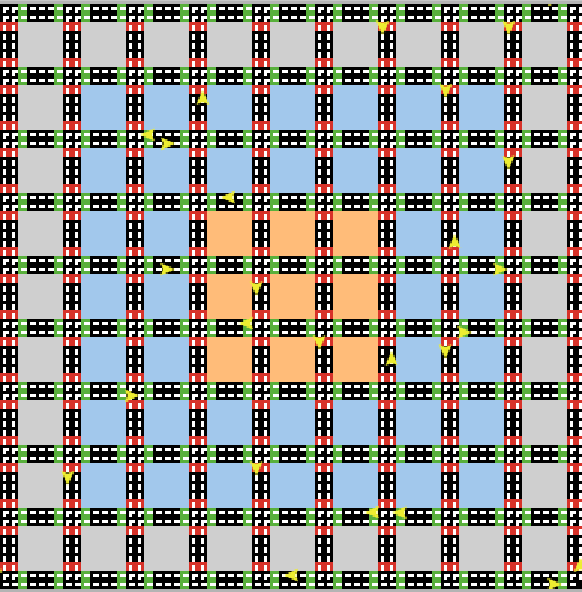
\includegraphics[width=6cm]{sections/pics/Taxi Cabs}
    \caption{Taxi Cab Model}
    \label{fig:taxi cab}
\end{figure}

Second example: the simulation is used in ~\cite{ismail2024software}.
In this study some rules, goals and tasks are listed, shown in figure~\ref{fig:tasktable} , that can be adapted and used in our model.
The NetLogo ui of this model is shown in figure~\ref{fig:a-ride}.
\begin{figure}
    \centering
    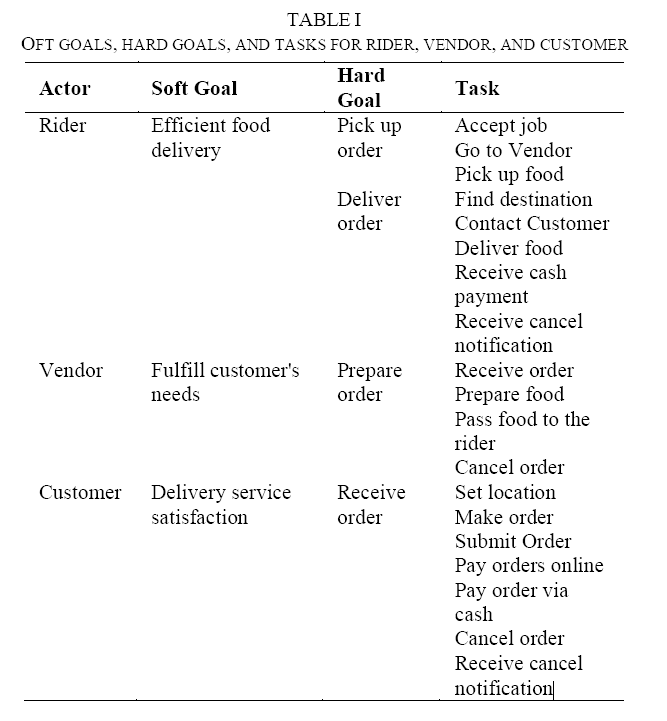
\includegraphics[width=8cm]{sections/pics/TaskTabel}
    \caption{Food Delivery}
    \label{fig:tasktable}
\end{figure}

\begin{figure*}
    \centering
    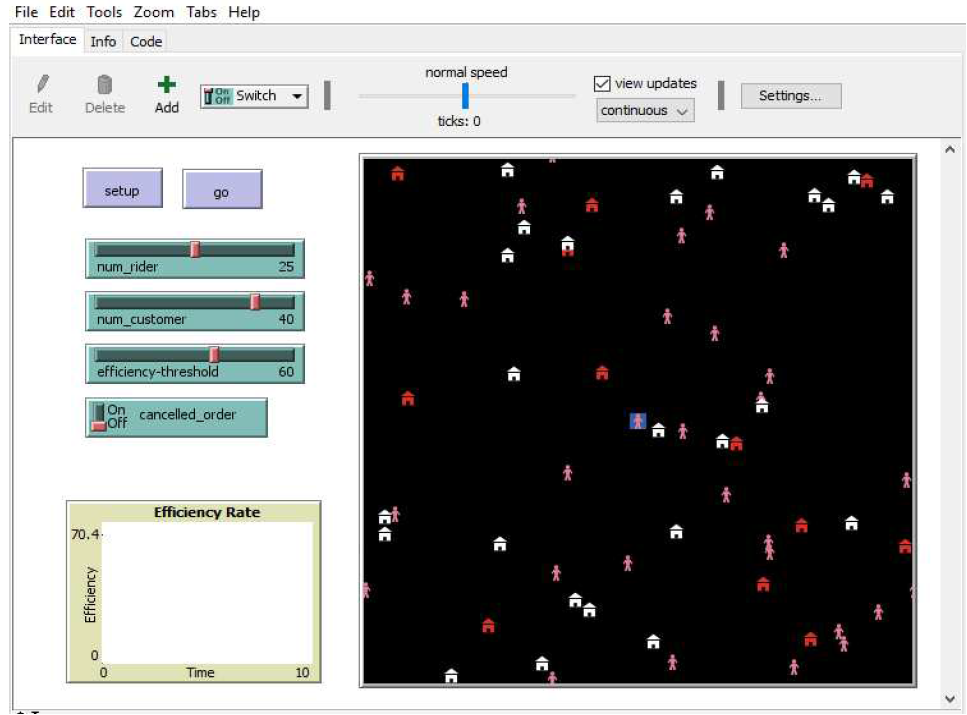
\includegraphics[width=\linewidth]{sections/pics/a-ride}
    \caption{NetLogo a-ride simulation}
    \label{fig:a-ride}
\end{figure*}


\section{Artefact}

The conceptional model has 3 types of agents:

-deliverers \\
-restaurants \\
-customers \\

There is one orchestrator, the delivery company, offers a website where customers can order,
restaurants pay the company a percentage of the delivery, they also offer means for the deliverers to
find deliveries and the shortest route.

Everything works on ticks of the clock, during 1 tick all agents execute one behaviour rule.
The order of execution among agents of one type is arbitrary.
This is interleaved execution, no parallelism.

%In the real world when ordering food, a customer will use the website from the delivery company to find a restaurant and place an order.
%The restaurant will take the order, the app
% Short telling how it works in the real world, Youtube

deliverers:
Start number can be set.
The deliverers get


restaurants:
the start number can be set, are placed at random
accept any orders, are open all the time,
prepare meals, the preparation time can be set,
after accepting a deliverer is asked.
when the meal is ready it can be picket up.
meals have properties, stage: preparation , waiting, on-route, delivered, discarded
A meal is only fresh for a time period.
If not picked up it wil be discarded.
Restaurants will leave the system if they have not enough orders.

customers:
order distribution, peek ours breakfast, lunch and  diner, once a week.
order from any restaurant they have no bad experience with
the price distribution, average can be set
they remember bad experiences for a certain time.
If delivered stale the customer is not satisfied and will not order from the restaurant also
it will order less food per week.







\begin{itemize}
    \item   The world consists op a grid of squares, some squares will be blocks of buildings and others represent the streets.
    \item   On this grid some predetermined restaurants and customers exist.
    \item   Customers will order food at a restaurant, the restaurant will prepare the food en will ask for a deliverer.
    \item   A deliverer will claim the delivery, move to the restaurant, pick the food up and move to the customer.
    \item   Agents may leave the world, i.e.,choose another delivery company, when unhappy.
    \item   Unhappiness will occur:
    \begin{itemize}
        \item   for customers when the food is not or too late delivered,
        \item   for restaurants when the food is not picked up or no orders are being placed,
        \item   for deliverers when they don't make any money.
    \end{itemize}
    \item    Calculating the profit for the delivery company.
    \item    The simulation consists of discreet steps, in which all agents simultaneous can do one thing.
    Some examples are:
    \begin{itemize}
        \item  move to the next square
        \item  place an order at a restaurant
        \item  do nothing
        \item  decide to take an order
    \end{itemize}
    \item   Behavior of the agents is rule based, these have to be programmed.
\end{itemize}


The environment where multiple agents act is called a multi-agent system end the problem is called a multi-agent planning problem (from~\cite{russell2016artificial}).
The research problem is actually a comparison between a system where there is one decision maker (the company assigns delivery jobs) and a system where each deliverer decide for its self (multiple decision makers).
This research will not be of a thoroughly theoretical nature though, its more of an exploratory/explanatory nature, see what happens under some conditions and explain the correlation.




\section{Results of simulations}


Consumers order meals from restaurants they like, if a meal is delivered cold they dislike the restaurant.
If they dont like the restaurant they will not place any orders anymore at that restaurant.

Restaurants create meals, if they dont get any orders for some time they quit.

The delivery provider make money for each order placed via their system, at the end they must have enough deliverers so that
customers keep ordering.
They have to pay the deliverers for the deliveries.



\subsection{Model variant 1}
Here come the results belonging to variant where deliverers are hired and paid an hourly wage.
The company destributes deliveries equally among the hired employees.
The company has to deside on how many to hire and for which periods.


\subsection{Model variant 2}
Here come the results where deliverers are independent contractors.
Deliverers come and go whenever they are pleased, like a open market.
Now deliverers have to deside to become a deliverer, deside to stop and to decide to go for a delivery.
To keep this simple, the meals are destributed among the available deliverers.
If a delivery person does not make enough many during a day they will quit.


\bibliography{references}

\bibliographystyle{icml2021}

\end{document}




